\vspace{10pt}
\section{Design Methodology}\label{sec:framwork}
Based on the analysis of Section~\ref{sec:w_and_r}, a new design flow are proposed to explore the design space of the cross-point ReRAM array. 

The proposed design flow are shown in Figure~\ref{fig:FlowChart}. Generally, the flow can be summarized as two stages: initialization stage and the computation stage. At the initialization stage, the physical parameters and the design constraints are firstly input. Based on physical parameters the coefficients matrix $A_{basic}$ and the vector of constant terms $C_{basic}$ are initialized. Since the $A_{basic}$ and $C_{basic}$ do not change with the different

\begin{figure}[!t]
\centering
  % Requires \usepackage{graphicx}
  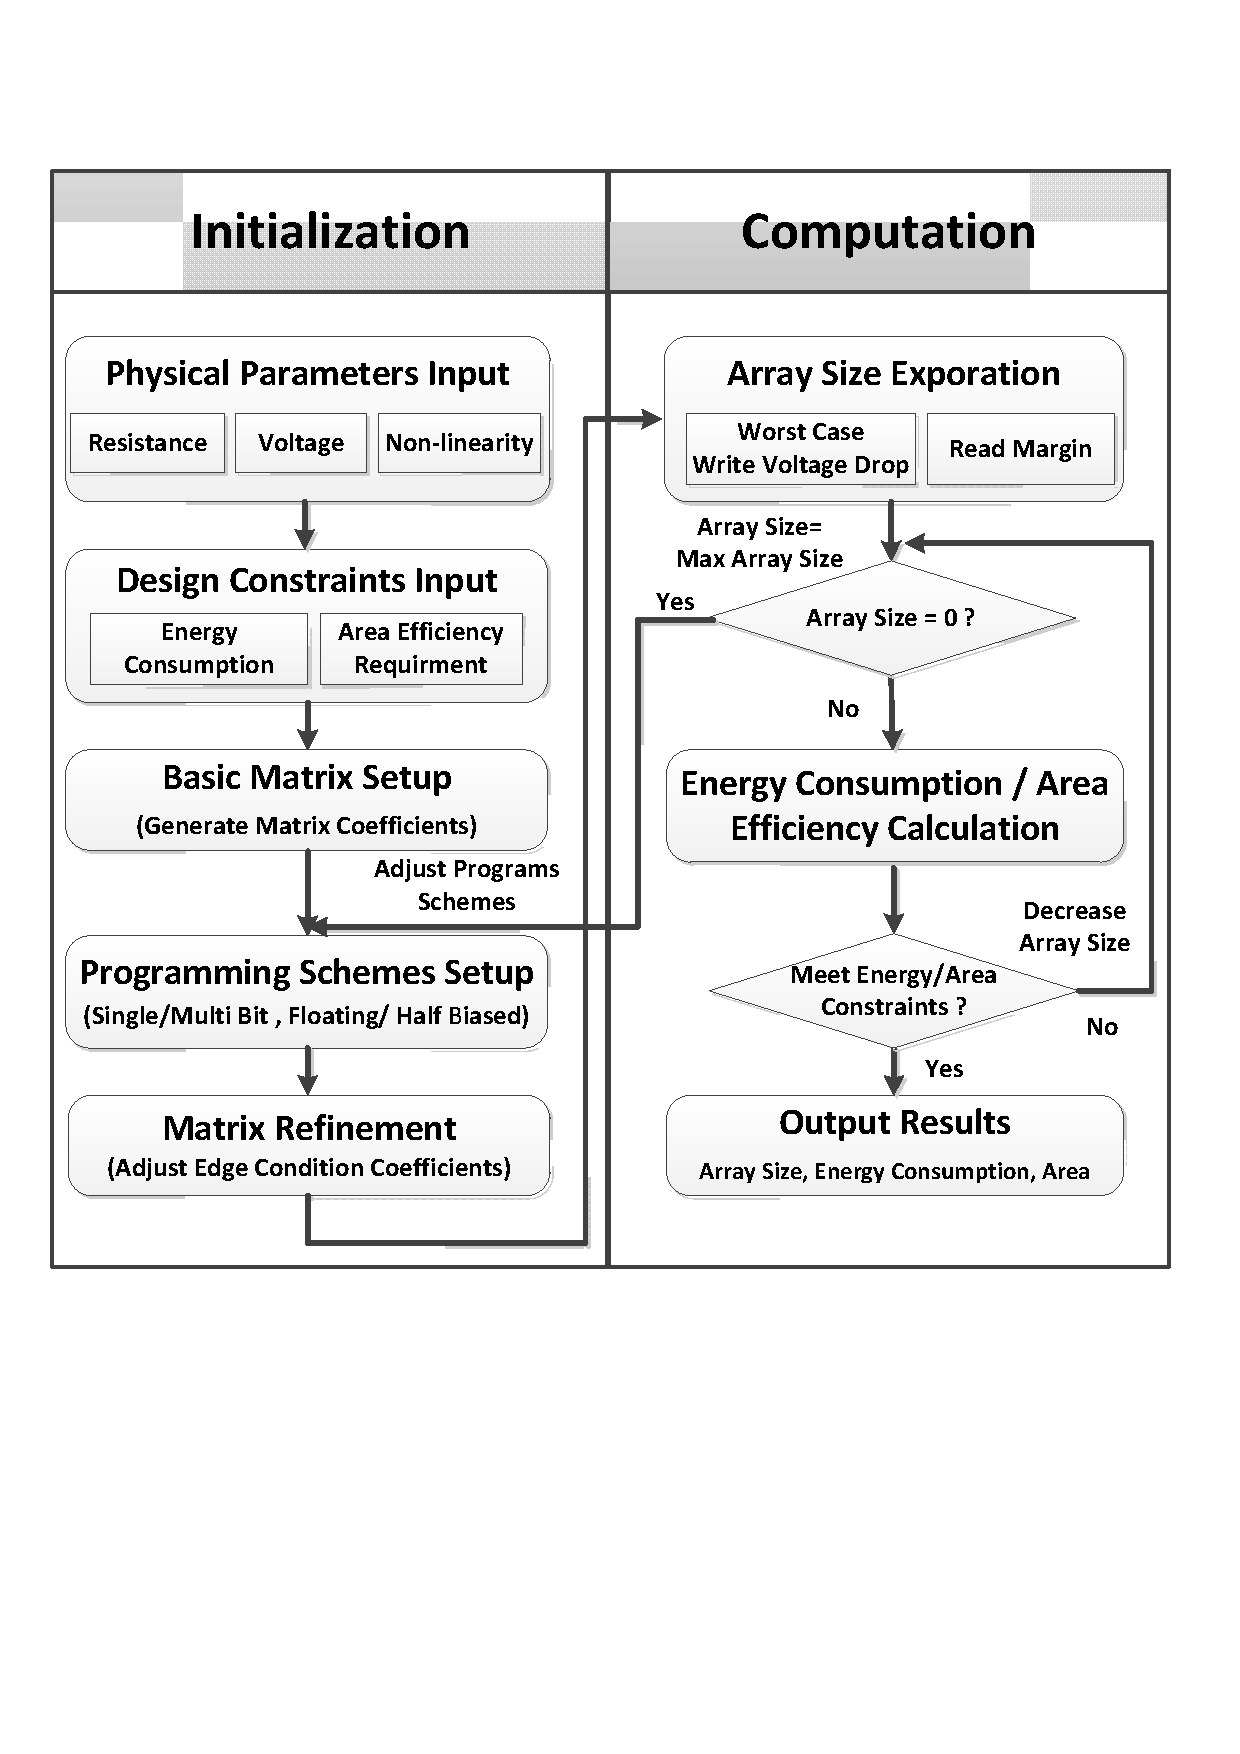
\includegraphics[width=0.5\textwidth]{./figures/FlowChart.pdf}\\
  \caption{The}\label{fig:FlowChart}
\end{figure}
